\documentclass{article}
\usepackage{cmap}
\usepackage[utf8]{inputenc}
\usepackage[english,ukrainian]{babel}
\usepackage{graphicx}
\usepackage{geometry}
\usepackage{listings}
\usepackage{indentfirst}
\usepackage{subfigure}
\usepackage{caption}
\usepackage{amsmath}
\geometry{
	a4paper,
	left=20mm,
	right=20mm,
	top=20mm,
	bottom=20mm
}
\lstset{
	extendedchars=\true,
	tabsize=4,
	language=python,
	showstringspaces=false,
	showtabs=false,
	frame=lrtb,
	columns=fixed,
	keepspaces,
	breaklines=true
}
\graphicspath{ {pictures} }
\setlength{\parindent}{4em}
\newcommand\subject{Чисельні методи}
\newcommand\lecturer{доцент кафедри ПЗ\\Мельник Н.Б.}
\newcommand\teacher{асистент кафедри ПЗ\\Гарматій Г.Ю.}
\newcommand\mygroup{ПЗ-16}
\newcommand\lab{9}
\newcommand\theme{Наближення функцій методом найменших квадратів}
\newcommand\purpose{Ознайомлення на практиці з методом найменших квадратів
	апроксимації (наближення) функцій}

\begin{document}
	\begin{large}
		\begin{titlepage}
			\thispagestyle{empty}
			\begin{center}
				\textbf{МІНІСТЕРСТВО ОСВІТИ І НАУКИ УКРАЇНИ\\
					НАЦІОНАЛЬНИЙ УНІВЕРСИТЕТ "ЛЬВІВСЬКА ПОЛІТЕХНІКА"}
			\end{center}
			\begin{flushright}
				Інститут \textbf{КНІТ}\\
				Кафедра \textbf{ПЗ}
			\end{flushright}
			\vspace{200pt}
			\begin{center}
				\textbf{ЗВІТ}\\
				\vspace{10pt}
				До лабораторної роботи № \lab\\
				\textbf{На тему}: “\textit{\theme}”\\
				\textbf{З дисципліни}: “\subject”
			\end{center}
			\vspace{90pt}
			\begin{flushright}
				
				\textbf{Лектор}:\\
				\lecturer\\
				\vspace{28pt}
				\textbf{Виконав}:\\
				
				студент групи \mygroup\\
				Коваленко Д.М.\\
				\vspace{28pt}
				\textbf{Прийняв}:\\
				
				\teacher\\
				
				\vspace{28pt}
				«\rule{1cm}{0.15mm}» \rule{1.5cm}{0.15mm} 2022 р.\\
				$\sum$ = \rule{1cm}{0.15mm}……………\\
				
			\end{flushright}
			\vspace{\fill}
			\begin{center}
				\textbf{Львів — 2022}
			\end{center}
		\end{titlepage}
		
		\begin{description}
			\item[Тема.] \theme.
			\item[Мета.] \purpose.
		\end{description}
		
		\section*{Теоретичні відомості}
		Розглянемо функцію $y=f(x)$, задану таблицею своїх значень $y_i=f(x_i)$ $i=\overline{0,n}$. Потрібно знайти поліном фіксованого $m$-го степеня ($m=\overline{0,n}$).
		\begin{gather}
			P_m(x)=a_0+a_1x+a_2x^2+...+a_mx^m\nonumber
		\end{gather}
		для якого похибкою апроксимації є середнє квадратичне відхилення
		\begin{gather}
			\sigma=\sqrt{\frac{1}{1+n}\sum_{i=0}^{n}(P_m(x_i)-y_i)^2}.\nonumber
		\end{gather}
		Оскільки поліном містить невизначені коефіцієнти $a_i$ $(i=\overline{0,m})$, то необхідно їх підібрати таким чином, щоб мінімізувати функцію
		\begin{gather}
			\varPhi(a_0,a_1,a_2,...,a_m)=\sum_{i=0}^{n}(P_m(x_i)-y_i)^2=\sum_{i=0}^{n}(\sum_{j=0}^{m}a_jx_i^j-y_i)^2\nonumber
		\end{gather}
		Використовуючи необхідну умову екстремуму $\frac{\partial\varPhi}{\partial a_k}=0$ $(k=\overline{0,m})$ функції від багатьох змінних $\varPhi(a_0,a_1,a_2,...,a_m)$, отримуємо так звану \textbf{нормальну систему} методу найменших квадратів для визначення коефіцієнтів $a_i$ $(i=\overline{0,m})$ апроксимаційного полінома
		\begin{gather}
			\sum_{j=0}^{m}(\sum_{i=0}^{n}x_i^{j+k})a_j=\sum_{i=0}^{n}y_ix_i^k,\hspace{28pt}k=\overline{0,m}\nonumber
		\end{gather}
		Отримана система - це система лінійних алгебраїчних рівнянь відносно невідомих $a_0,a_1,a_2,...,a_m$.
		
		\section*{Лабораторне завдання}
		Методом найменших квадратів побудувати лінійний, квадратичний і
		кубічний апроксимаційні поліноми для таблично заданої функції.
		\vspace{5pt}
		
		\begin{tabular}{|c|c|c|c|c|c|c|}
			\hline
			x & 4.03 & 4.08 & 4.16 & 4.23 & 4.26 & 4.33\\
			\hline
			y & 2.8 & 2.94 & 3.2 & 3.38 & 3.53 & 3.75\\
			\hline
		\end{tabular}
	
		\section*{Хід роботи}	
		Нормальна система рівнянь для визначення коефіцієнтів лінійного полінома має такий вигляд:
		\begin{gather}
			\left\{\begin{array}{@{}l@{}}
				\displaystyle(n+1)a_0 + (\sum_{i=0}^{n}x_i)a_1= \sum_{i=0}^{n}y_i\\\nonumber
				\displaystyle(\sum_{i=0}^{n}x_i)a_0 + (\sum_{i=0}^{n}x_i^2)a_1= \sum_{i=0}^{n}y_ix_i\\\nonumber
			\end{array}\right.\,
		\end{gather}
		Підставивши значення таблично заданої функції отримаю:
		\begin{gather}
			\left\{\begin{array}{@{}l@{}}
				6a_0 + 25.09a_1= 19.6y_i\\\nonumber
				25.09a_0 + 104.98a_1= 82.16y_ix_i\nonumber
			\end{array}\right.\,
		\end{gather}
		Розв'язавши систему отримаю розв'язки $-9.95$ та $3.16$.
			
		\noindent\textit{\textbf{Код програми} (файл lab\_\lab1.py):}
		\begin{lstlisting}
import numpy as np
from scipy.linalg import solve

def data_to_matrix(path):
	return (
		np.loadtxt(open(path, "rb"), delimiter=",")[0],
		np.loadtxt(open(path, "rb"), delimiter=",")[1],
	)

def normal_system_of_equations(x, y, m):
	return (
		np.array([[sum([x**(i+j) for x in x]) for i in range(m+1)] for j in range(m+1)]),
		np.array([sum(map(lambda y,x: y * x**i, y, x)) for i in range(m+1)])
	)

def gauss_method(A, n):
	for i in range(n):
		for j in range(n):
			if i != j:
				ratio = A[j][i]/A[i][i]
				for k in range(n + 1):
					A[j][k] -= ratio * A[i][k]
	return [A[i][n]/A[i][i] for i in range(n)]

path = input("Введіть шлях до файлу з даними: ") or "data.csv"
x, y = data_to_matrix(path)

a, b = normal_system_of_equations(x, y, 1)
print(f"Лінійний: \t {[round(x, 4) for x in solve(a, b)]}")
a, b = normal_system_of_equations(x, y, 2)
print(f"Квадратичний: \t {[round(x, 4) for x in solve(a, b)]}")
a, b = normal_system_of_equations(x, y, 3)
print(f"Кубічний: \t {[round(x, 4) for x in solve(a, b)]}")\end{lstlisting}
		
		\noindent\textit{\textbf{Файл даних} (data.csv):}
		\begin{lstlisting}
4.03, 4.08, 4.16, 4.23, 4.26, 4.33
2.8, 2.94, 3.2, 3.38, 3.53, 3.75\end{lstlisting}
		
		\begin{figure}[h!]
			\centering
			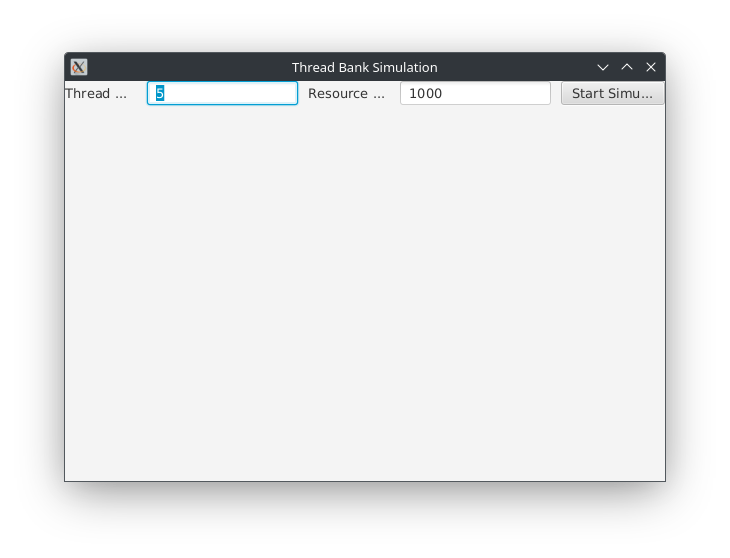
\includegraphics[scale=1]{1}
			\caption{Робота програми}
		\end{figure}
		
		\section*{Висновок}
		На лабораторній роботі я засвоїв практичні навички використання методу найменших квадратів для побудови лінійного, квадратичного і
		кубічного апроксимаційного полінома для таблично заданої функції
		
		\begin{tabular}{|c|c|c|c|c|c|c|}
			\hline
			x & 4.03 & 4.08 & 4.16 & 4.23 & 4.26 & 4.33\\
			\hline
			y & 2.8 & 2.94 & 3.2 & 3.38 & 3.53 & 3.75\\
			\hline
		\end{tabular}
		\vspace{5pt}\\
		та отримав такий результат результат:
		\begin{list}{}{}
			\item [Лінійний:] $P_1(x) = -9.9538 + 3.1615x$;
			\item [Квадратичний:] $P_2(x) = 11.0148 - 6.8864x + 1.203x^2$;
			\item [Кубічний:] $P_3(x) = -137.0988 + 99.3769x - 24.2008x^2 + 2.0237x^3$.
		\end{list}
		\begin{figure}[!htb]
			\minipage{0.32\textwidth}
			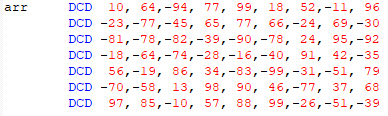
\includegraphics[width=\linewidth]{2}
			\caption{Лінійний}\label{fig:2}
			\endminipage\hfill
			\minipage{0.32\textwidth}
			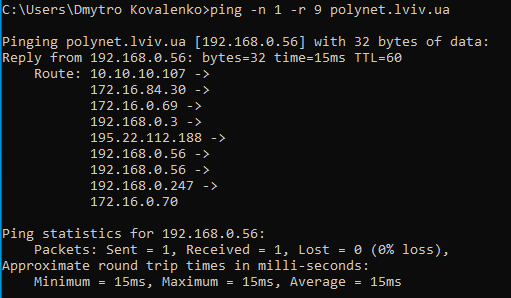
\includegraphics[width=\linewidth]{3}
			\caption{Квадратичний}\label{fig:3}
			\endminipage\hfill
			\minipage{0.32\textwidth}%
			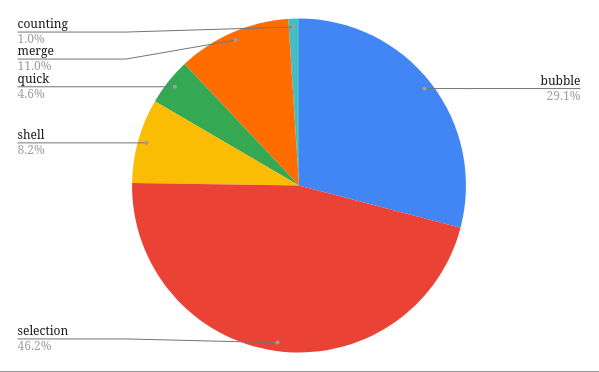
\includegraphics[width=\linewidth]{4}
			\caption{Кубічний}\label{fig:4}
			\endminipage
		\end{figure}

	\end{large}
\end{document}
